\section{Discussion}
\label{sec:discussion}



In this section, we offer perspectives on \genco's performance and discuss its practical deployment. Future research directions for \genco and the GridFM Development Framework are provided in \cref{appendix:future_work}.

\paragraph{Performance of \genco.}
\genco's performance results are summarized in \cref{fig:summary_plot}, which illustrates semi-quantitatively the computational speed and solution accuracy of DC solvers and \genco relative to classical AC solvers. 
\genco offers a middle ground: In contrast to AC solvers and DC approximations, \genco sustains high throughput while recovering the full set of grid variables, including voltage magnitudes and reactive power.  
For PF on grids with $\geq 2000$ bus nodes, runtime improvements of \maxpfspeedups w.r.t. AC-PF at residuals comparable to DC solvers (\cref{tab:pf_selected_genco_tradeoff}) were achieved. For OPF, the speedups are larger, reaching \maxopfspeedups for case~2000 w.r.t. AC-OPF (\cref{fig:gridsize_runtime_opf}) at optimality gaps $\leq 0.3\%$, and feasibility within 0.35\% of the mean bounds on the OPFData benchmark (\cref{tab:opf_results}).
For SE, \genco can even outperform the weighted least squares (WLS) method (\cref{fig:perturbation}). Its runtime advantage grows with the number of outliers, as classical SE requires additional iterations to process them. Further, \genco always returns a high-quality estimate even when WLS fails to converge. 
Compared to task-specific machine learning models, \genco reached state-of-the-art performance across all three steady-state grid tasks, at a fraction of development time and costs, due to the unified architecture acting as a common backbone, sharing model and learning parameters, so hyperparameter optimization is required only once, rather than repeated for every task. Further task-specific optimization remains possible but was not required to achieve competitive performance.



\begin{figure}
    \centering
    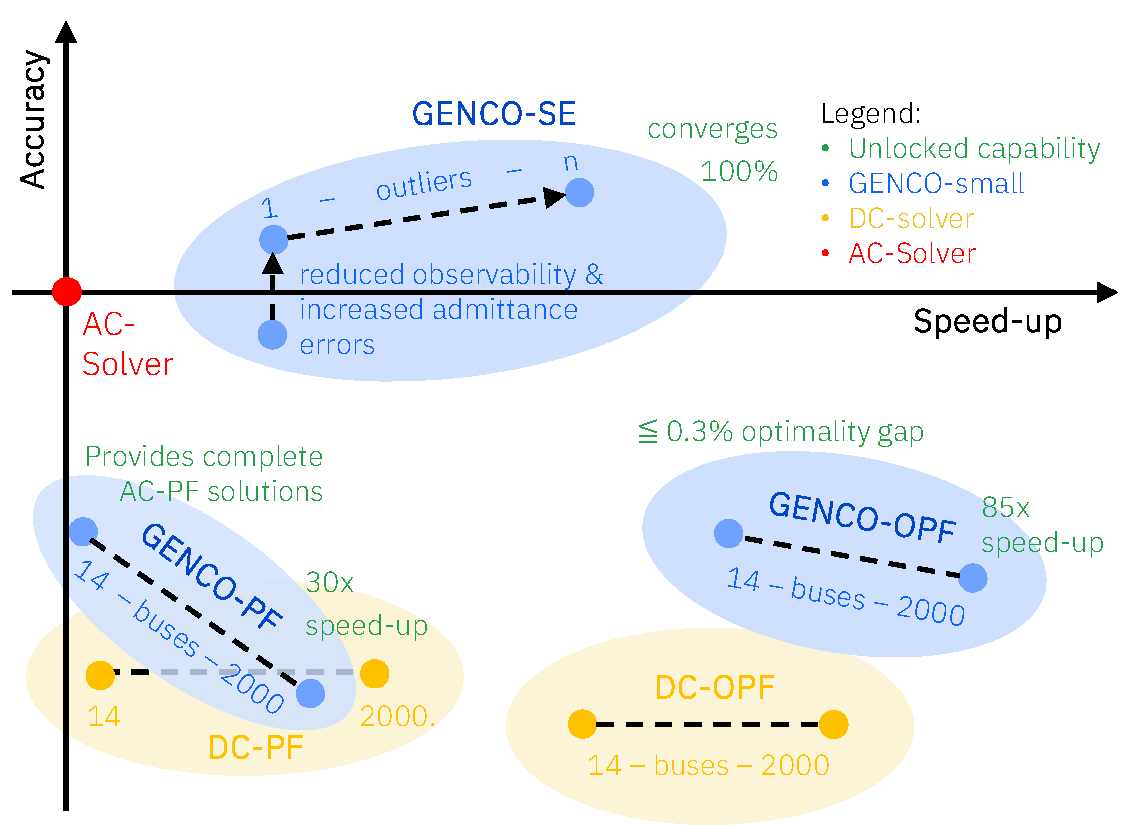
\includegraphics[width=1.0\linewidth]{figures/discussion/genco_Performance_Summary_Plot_V8.pdf}
    \caption{Semi-quantitative performance summary comparing \genco and classical DC solvers relative to classical AC solvers. Specific \genco capabilities are highlighted explicitly.}
    \label{fig:summary_plot}
\end{figure}

\paragraph{Deployment of \genco.}
% As motivated above, \genco is intended to complement classical solvers for providing fast OPF or SE and fast \textit{batched} PF for large grids. 
Our validation of \genco-PF on the real-world HQ1200 grid topology (\cref{tab:hq1200_results}) and SCADA data (\cref{fig:hq_scada_finetune}) indicates that pretraining \genco on synthetic \datakit data, followed by fine-tuning on approximately 15k data points (one year of SCADA data at 30-minute intervals), is important for achieving similar accuracy to DC solvers. We also showed that pretraining on a large number of different grids allows reaching similar accuracy as DC-PF with very few samples (\cref{subsubsec:transfer}). Further, we envision a safeguarded hybrid workflow in which \genco rapidly evaluates all scenarios, while power-balance residuals and violation checks identify critical cases for re-evaluation with a classical AC solver. With appropriate screening criteria, this substantially increases throughput while preserving numerical reliability, as most scenarios avoid a full AC solve.
% The result is a secure and scalable assessment across ensembles that prevents unphysical or erroneous predictions from propagating downstream.



\paragraph{Standardized development and benchmarking.}
With the release of the GridFM Development Framework---\datakit, \graphkit, and the accompanying datasets (\cref{fig:motivational_example})---we establish an end-to-end pipeline for reproducible neural solver development and benchmarking across the three steady-state grid analysis tasks. A new model only needs to be implemented as a single class in \graphkit to take advantage of the shared data-loading, preprocessing, training, and evaluation routines. The widely used \pfdelta and OPFData benchmarks enable baseline comparison against state-of-the-art models, whereas \datakit data allows robustness assessments with user-defined perturbations including OPF scenarios with variable generator costs and topology variants beyond N-2. In addition, robustness assessments of neural solvers require more than reporting only mean or median errors. Instead, the full error distribution must be reported, as supported by \graphkit. 

\paragraph{Fair runtime analysis methodology.}
In \cref{subsec:scaling}, we proposed a protocol for a fair comparison of neural solvers against one another and against classical solvers, based on batched inference with fully utilized GPUs and CPUs of the same hardware generation. To our knowledge, all prior studies compare GPU inference against a single classical-solver thread on one core, which does not reflect the capacity of modern multi-core processors and the typical batch processing in power systems. For runtime evaluation, the model must first be integrated into \graphkit. The user can then specify whether data loading from disk should be included in the reported runtime or isolated from the solver execution. The benchmarking script automatically initializes the classical and neural solvers, determines suitable worker counts and batch sizes, executes the benchmark runs, and reports the resulting runtime metrics.





\section{Conclusion}
\label{sec:conclusion}

Our unified neural solver and open-source GridFM Development Framework represent two technical contributions: (i) an end-to-end workflow that enables fair and reproducible neural solver development and benchmarking, and (ii) \genco, a state-of-the-art neural solver that unifies the three fundamental steady-state grid analysis tasks within a single shared representation. Together, these contributions enable the power-system-AI community to compare models on a common foundation and accelerate innovation.\\ %They further support safeguarded hybrid workflows that achieve orders-of-magnitude speed-ups without compromising accuracy, convergence, or grid-variable completeness, all within a low-code environment. As such, they can play an important role in enabling the rapid energy transition, which requires probabilistic grid assessments at unprecedented scale, and represent a first step toward foundation models for the electric grid.\\

These contributions directly address the four key challenges for neural solvers identified in \cref{sec:related}:\\

First, we responded to the challenge of a \textit{unified grid representation and architecture} through a shared graph representation in which task-specific differences in the input features are covered by masking: irrelevant variables are hidden, while unknown and decision variables are exposed for inference, yielding a fixed input representation across tasks. The heterogeneous graph structure, neural architecture, normalization scheme, and AC-physics enforcement remain unchanged, with only lightweight, non-learnable task-specific physics decoders added. Consequently, the same model and hyperparameters serve PF, OPF, and SE, enabling direct transfer of architectural improvements and tuning effort while reducing the time and compute cost required for model training.\\

Second, \genco addresses the \textit{runtime--feasibility--optimality--completeness trade-off} through physics-based solution completion and iterative correction with power-balance feedback that scales linearly with grid size, while preserving efficient batched inference. This places \genco between classical AC and DC solvers: it approaches the speed of DC methods while recovering the full set of AC variables, enabling fast approximate AC solutions. On large grids, \genco achieves up to \maxpfspeedups speedups over Newton--Raphson for PF while attaining residual levels comparable to DC-PF. For OPF, it provides up to \maxopfspeedups speedups over IPOPT while maintaining an optimality gap of $\leq 0.3\%$ on the OPFData benchmark. For SE, it consistently returns high-quality estimates, including in cases where WLS fails to converge.\\

Third, \genco's \textit{generalization} is evaluated with \datakit, which extends existing sampling methods with realistic load profiles, higher-order topology perturbations beyond N-2, and admittance variations, adding out-of-limit operating points for PF, generator cost variations for OPF, and sparse, noisy, and mismatched measurements for SE. \genco generalizes to contingencies up to N-20 with up to $3\times$ lower median residuals than DC-PF, and remains robust to out-of-operating-limit scenarios, outperforming DC-PF on line-loading prediction while also detecting voltage violations. Most importantly, we assess \genco on the real-world HQ1200 grid topology and its SCADA-derived states, achieving similar performance to DC-PF. Topology-agnostic zero-shot transfer remains unsolved: the pretrained \genco requires fine-tuning on roughly $1{,}000$ grid-specific samples to outperform DC-PF on a new grid.\\

Finally, we address \textit{workflow and evaluation fragmentation} along three axes: (i) we enable harmonized comparisons across datasets by evaluating \genco on \pfdelta and OPFData and providing converters that map existing benchmarks into \datakit, while releasing standardized PF, OPF, and SE datasets on Hugging Face; (ii) we introduce a method for fair runtime benchmarking on fully utilized CPUs and GPUs, based on amortized accounting for hardware and parallelization effects; and (iii) we release the Linux Foundation OpenGridFM libraries (\datakit and \graphkit) as a shared backbone that enables model development and utilization across PF, OPF, and SE tasks, in a low-code environment. %In addition, we provide guidance on how to apply \genco to new grid topologies with abundant or scarce SCADA data, and we describe hybrid workflows that deliver assessments at speed without compromising accuracy, respecting the safety requirements of grid operations and planning. \\









\begin{table}
\centering
\small
\caption{Author contributions.}
\label{tab:contributions}
\begin{tabularx}{\linewidth}{>{\bfseries}l X}
\hline
Contribution & Authors \\
\hline
Conceptualization &
Alban Puech, Matteo Mazzonelli, Jonas Weiss, François Mirallès, Hendrik F.~Hamann, Etienne Vos, Thomas Brunschwiler \\
\hline
Experiments &
Alban Puech, Matteo Mazzonelli, Tamara R.~Govindasamy, Mangaliso Mngomezulu, Héctor Maeso García, Thomas Tolhurst, Javad Bayazi, Ali Moeini, Naomi Simumba, David Nelischer, Etienne Vos, Thomas Brunschwiler \\
\hline
Software Engineering &
Thomas Tolhurst, Javad Bayazi, Celia Cintas, Romeo Kienzler \\
\hline
Writing &
Alban Puech, Tamara R.~Govindasamy, Mangaliso Mngomezulu, François Mirallès, Hendrik F.~Hamann, Etienne Vos, Thomas Brunschwiler \\
\hline
Editing \& Reviewing &
Alban Puech, Florian Dörfler, Gabriela Hug, Martin Mevissen, Juan Bernabé-Moreno, François Mirallès, Hendrik F.~Hamann, Etienne Vos, Thomas Brunschwiler \\
\hline
Supervision &
Alban Puech, Jonas Weiss, Anna Varbella, Florian Dörfler, Gabriela Hug, Etienne Vos, Thomas Brunschwiler \\
\hline
Project Management &
Alban Puech, Jonas Weiss, Martin Mevissen, Juan Bernabé-Moreno, François Mirallès, Hendrik F.~Hamann, Etienne Vos, Thomas Brunschwiler \\
\hline
Sponsoring &
Juan Bernabé-Moreno, François Mirallès, Hendrik F.~Hamann \\
\hline
\end{tabularx}
\end{table}


\section*{Acknowledgments}

This work was partially supported by the U.S. Department of Energy’s Office of Critical Minerals and Energy Innovation (CMEI), Integrated Energy Systems Office (IESO), under the project titled “Artificial Intelligence for Energy Dominance,” Award Number 54805. We thank Panagiotis Grontas for proofreading the paper, and Mohammad Atif, Guang Zhao, Benedikt Wahl, Riccardo Ghetti, Srihith Bharadwaj Burra, Tilman Bockhacker, Olayiwola Arowolo, and Antonio Alcántara for their feedback and contributions to \graphkit and \datakit. We also thank Matteo Baù, Marcus Freitag, Johannes Schmude, Le Xie, and Thomas Theis for their valuable comments, insights, and discussions. Finally, the authors acknowledge valuable discussions with the GridFM community.



\section*{Author Contributions}
Author contributions are summarized in \cref{tab:contributions}.

\section*{Declaration of Interests}
The authors declare no competing interests.

\section*{Declaration of Generative AI and AI-Assisted Technologies}
During the preparation of this work, the authors used ChatGPT and Claude to find more concise reformulations and to condense paragraphs. After using these tools, the authors reviewed and edited the content as needed and take full responsibility for the content of the publication.